\section{Recommender Systems}

\begin{frame}
	\makebox[\linewidth]{
		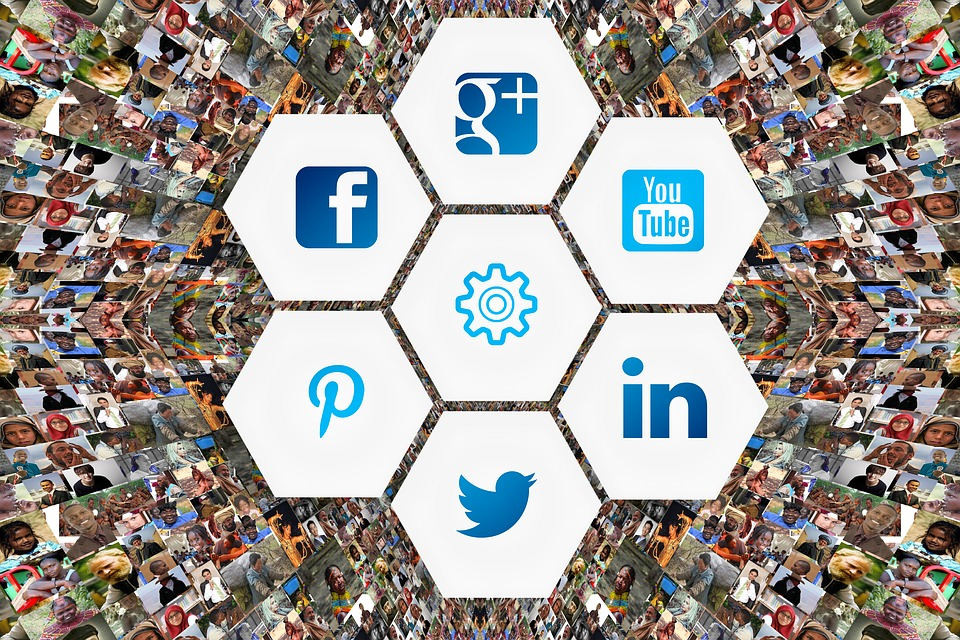
\includegraphics[width=\columnwidth,height=\paperheight,keepaspectratio]{../pictures/social_media.jpeg}}
\end{frame}
% recommender systems are everywhere around us.

\begin{frame}{Recommender Systems in Communication Science}  
	\begin{block}{New research questions}
		\begin{enumerate}
			\item<2-> \alert{Political communication and journalism}. E.g., to craft personalized news diets. This may have, however, consequences for the diversity of news diets and for democracy \parencite{Moller2018, Locherbach2018}
			\item<3-> \alert{Organizational and corporate communication}. E.g., applications in the field of hiring and recruitment.
			\item<4-> \alert{Persuasive communication}. E.g., in the health domain--recommendation algorithms for tailored health interventions \parencite{Kim2019}
			\item<5-> \alert{Entertainment communication}. E.g., movie recommenders
				\end{enumerate}
	\end{block}
\end{frame}

\begin{frame}{Recommender Systems} 
\begin{block}{Two central problems within Recommender Systems}
	\begin{enumerate}
		\item<2-> \alert{Predicting problem}. Typical problem involves a lot of missing data (e.g., user only rated a small subset of movies/news articles/ etc.) How can we deal with missing data? 
		\item<3-> \alert{Ranking problem}.  Given \textit{n} items, can we identify the top \textit{k} items to recommend?
	\end{enumerate}
\end{block}
\only<4->{These problems are not isolated; rather, they are connected. }
\end{frame}

\begin{frame}{Recommender Systems} 
\begin{block}{How do recommender systems learn?}
	\begin{enumerate}
		\item<2-> \alert{Explicit user preferences}. Ratings or responses 
		\item<3-> \alert{Implicit user preferences}. E.g., clicks or viewing time
		\item<3-> \alert{Content}. E.g., based on text similarity techniques
	\end{enumerate}
\end{block}
\end{frame}

\begin{frame}{Recommender Systems} 
\begin{block}{Types of recommender systems  \parencite{Wieland2021, Locherbach2018, Moller2018}}
	\begin{enumerate}
		\item 'Basic' knowledge-base recommender systems
		\item Content-based recommender systems
		\item Collaborative  recommenders 
	\end{enumerate}
\end{block}{\tiny }
\end{frame}

\section[Knowledge-based RecSys]{Knowledge-based Recommender Systems}
\begin{frame}{Knowledge-based recommender system} 
\begin{block}{When to use?}
	\begin{itemize}
		\item<2-> To overcome the \textbf{cold start problem}; when we do not have ratings of individual users. 
		\item<3-> Simple model. It does not rely on user's explicit or implicit ratings, but on specific queries.
		\item<4-> Typical use case: Real-estate. Buying a house is, for most families, a rare/ single event. 
	\end{itemize}
\end{block}
\end{frame}

% This prints the bibliography on the slide
%\section{An example with some Python code\dots}

\begin{frame}
\makebox[\linewidth]{
	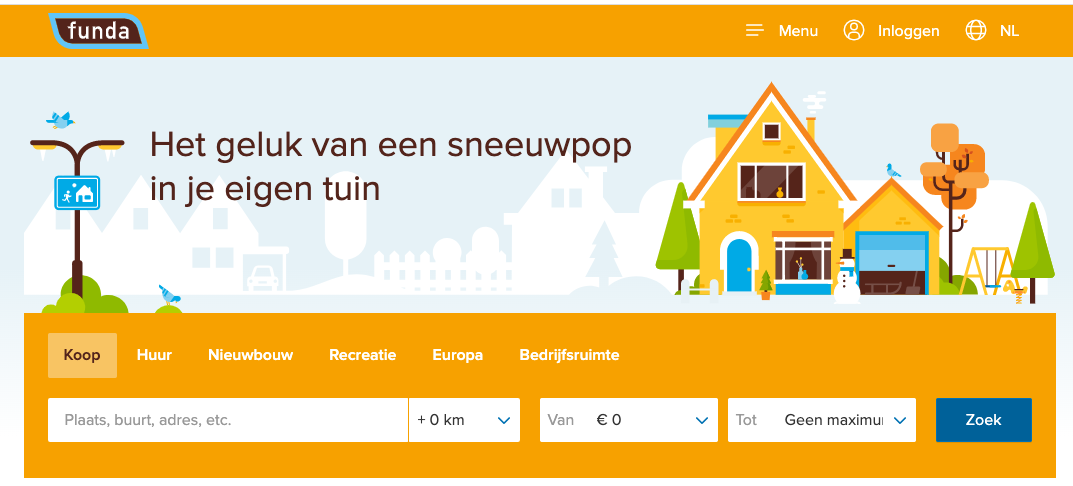
\includegraphics[width=\columnwidth,height=\paperheight,keepaspectratio]{../pictures/funda}}
\end{frame}

\begin{frame}{Use case: ImDb database}
\makebox[\linewidth]{
	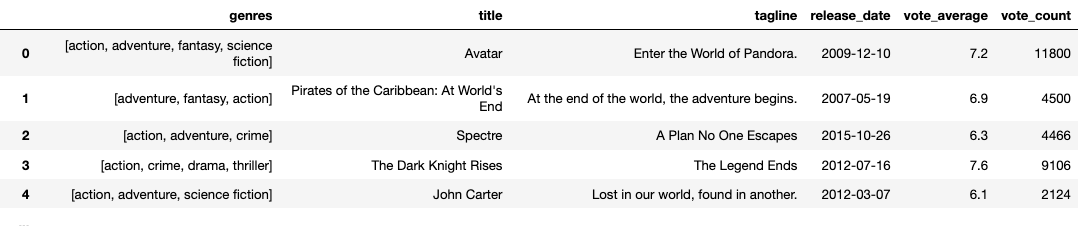
\includegraphics[width=\columnwidth,height=\paperheight,keepaspectratio]{../pictures/data}}
\end{frame}

\question{What are relevant variables to use in a knowledge-based recommender system?}

\begin{frame}[fragile]{Knowledge-based recommender system}
How can we work with user input without a front-end (such as the website of funda? 
\pause
$\rightarrow$ enter python's native \alert{input()} function.
\pause
\begin{minted}{python}
print("What is your favorite movie genre?")
genre = input()
\end{minted}
\pause
\begin{lstlistingoutput}
what is your favorite movie genre?
[...]
\end{lstlistingoutput}
\end{frame}


\begin{frame}[fragile]{Improving knowledge-based recommender system}
\begin{block}{When to use?}
	\begin{itemize}
		\item <1-> It is important to think about ways to make the recommendation relevant for individuals
		\item <2-> Do you have more information in your db that make your top-listed recommendations as relevant as possible?
	\end{itemize}
\end{block}
\pause
\begin{minted}[fontsize=\footnotesize]{python}
recommend_movies = movies.sort_values('vote_average', ascending=False)
\end{minted}
\end{frame}

\section[Content-based RecSys]{Content-based Recommender Systems}

\begin{frame}
	\begin{block}{Content-based systems}
		\begin{itemize}
			\item <1-> Recommends items based on user's profiles. 
			\item <2-> Profiles are based on e.g., ratings, and represents user's tasts/ preferences. 
			\begin{itemize}
				\item <3-> For example, how often a user has clicked on, or liked, a movie. 
			\end{itemize}
			\item <4-> Recommendation is based on \alert{similarity} beween items in the content.
			\begin{itemize}
				\item <5-> Content is here: e.g., genre, tags, plot, authors, directors, location, etc. 
			\end{itemize}
		\end{itemize}
	\end{block}
\end{frame}

\begin{frame}{Example of a content-based recsys}
	\makebox[\linewidth]{
		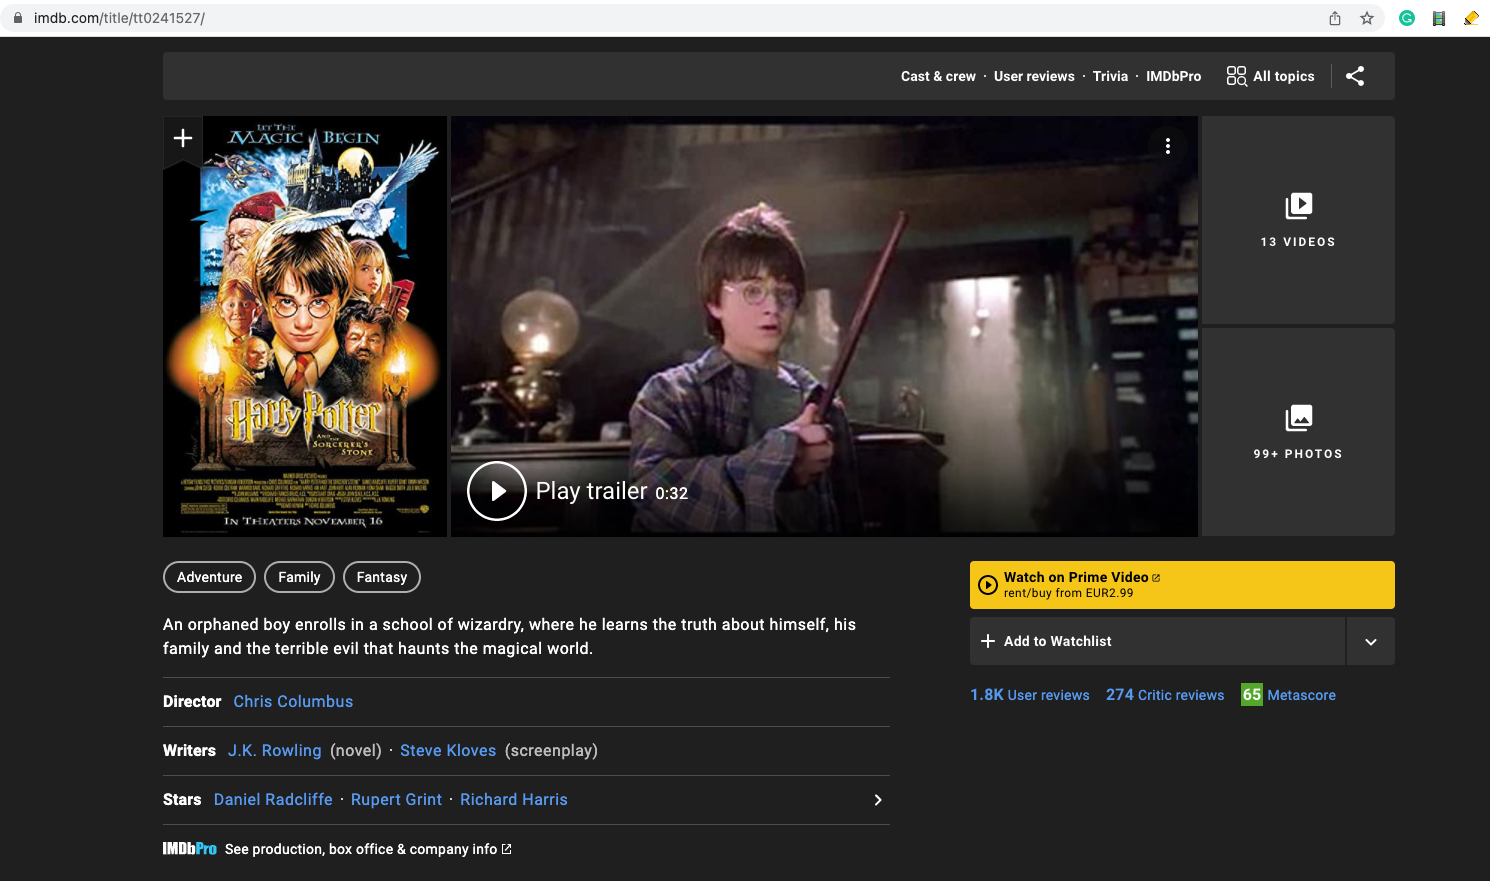
\includegraphics[width=\columnwidth,height=\paperheight,keepaspectratio]{../pictures/harry1.png}}
\end{frame}

\begin{frame}{Example of a content-based recsys}
	\makebox[\linewidth]{
		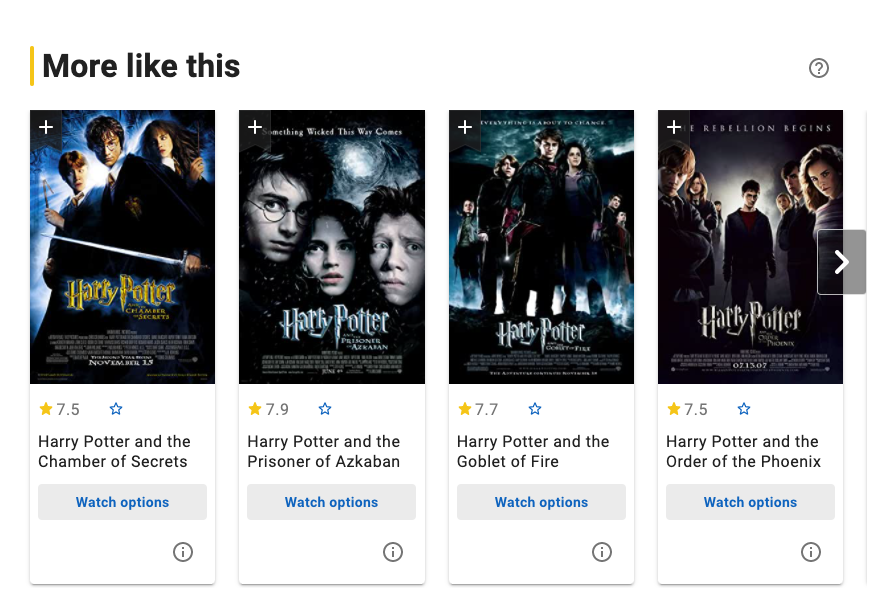
\includegraphics[width=\columnwidth,height=\paperheight,keepaspectratio]{../pictures/harry2.png}}
\end{frame}

%as you can see, it works quite well, but also has its drawbacks.. can be quite obvious.

%using information of the items themselves, rather than the aggregate user data. Even for more advanced recommender systems, baking in some knowledge about the content can be very helpful. 

%The movielens dataset does not give us a lot of information, but it does 

%Let's have a look again at the MovieLens dataset. If we know given user likes a specific genre, the user might also like other genres. In addition, we can use year of release. We can narrow it down further to movies that are close to a specific release data. 
% there is all sort of information availabe here, that we might use. 

\begin{frame}{Use case: ImDb database}
	Let's have a look at our use case again. \\
	Are there attributes that you could use to estimate similarity in movies?
	\makebox[\linewidth]{
		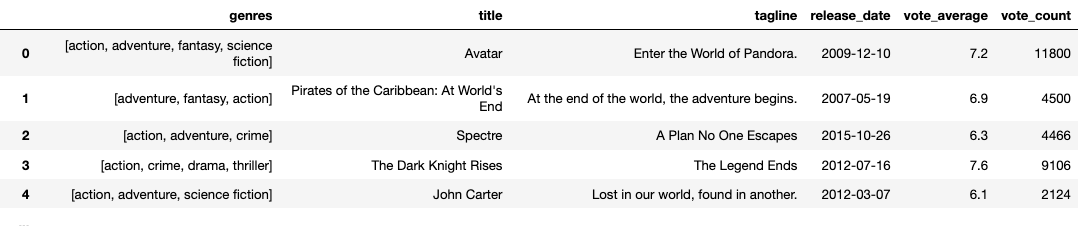
\includegraphics[width=\columnwidth,height=\paperheight,keepaspectratio]{../pictures/data}}
\end{frame}

% how can we calculate similarity, just based on genre?
% Cosine is very handy, not only for textule data, but also for different types of numeric data. 

% to make it easier to understand, lets imagine that every movie has only one of the follwoing genres: 
%romance or comedy

\begin{frame}{Similarity between movies}
	\makebox[\linewidth]{
		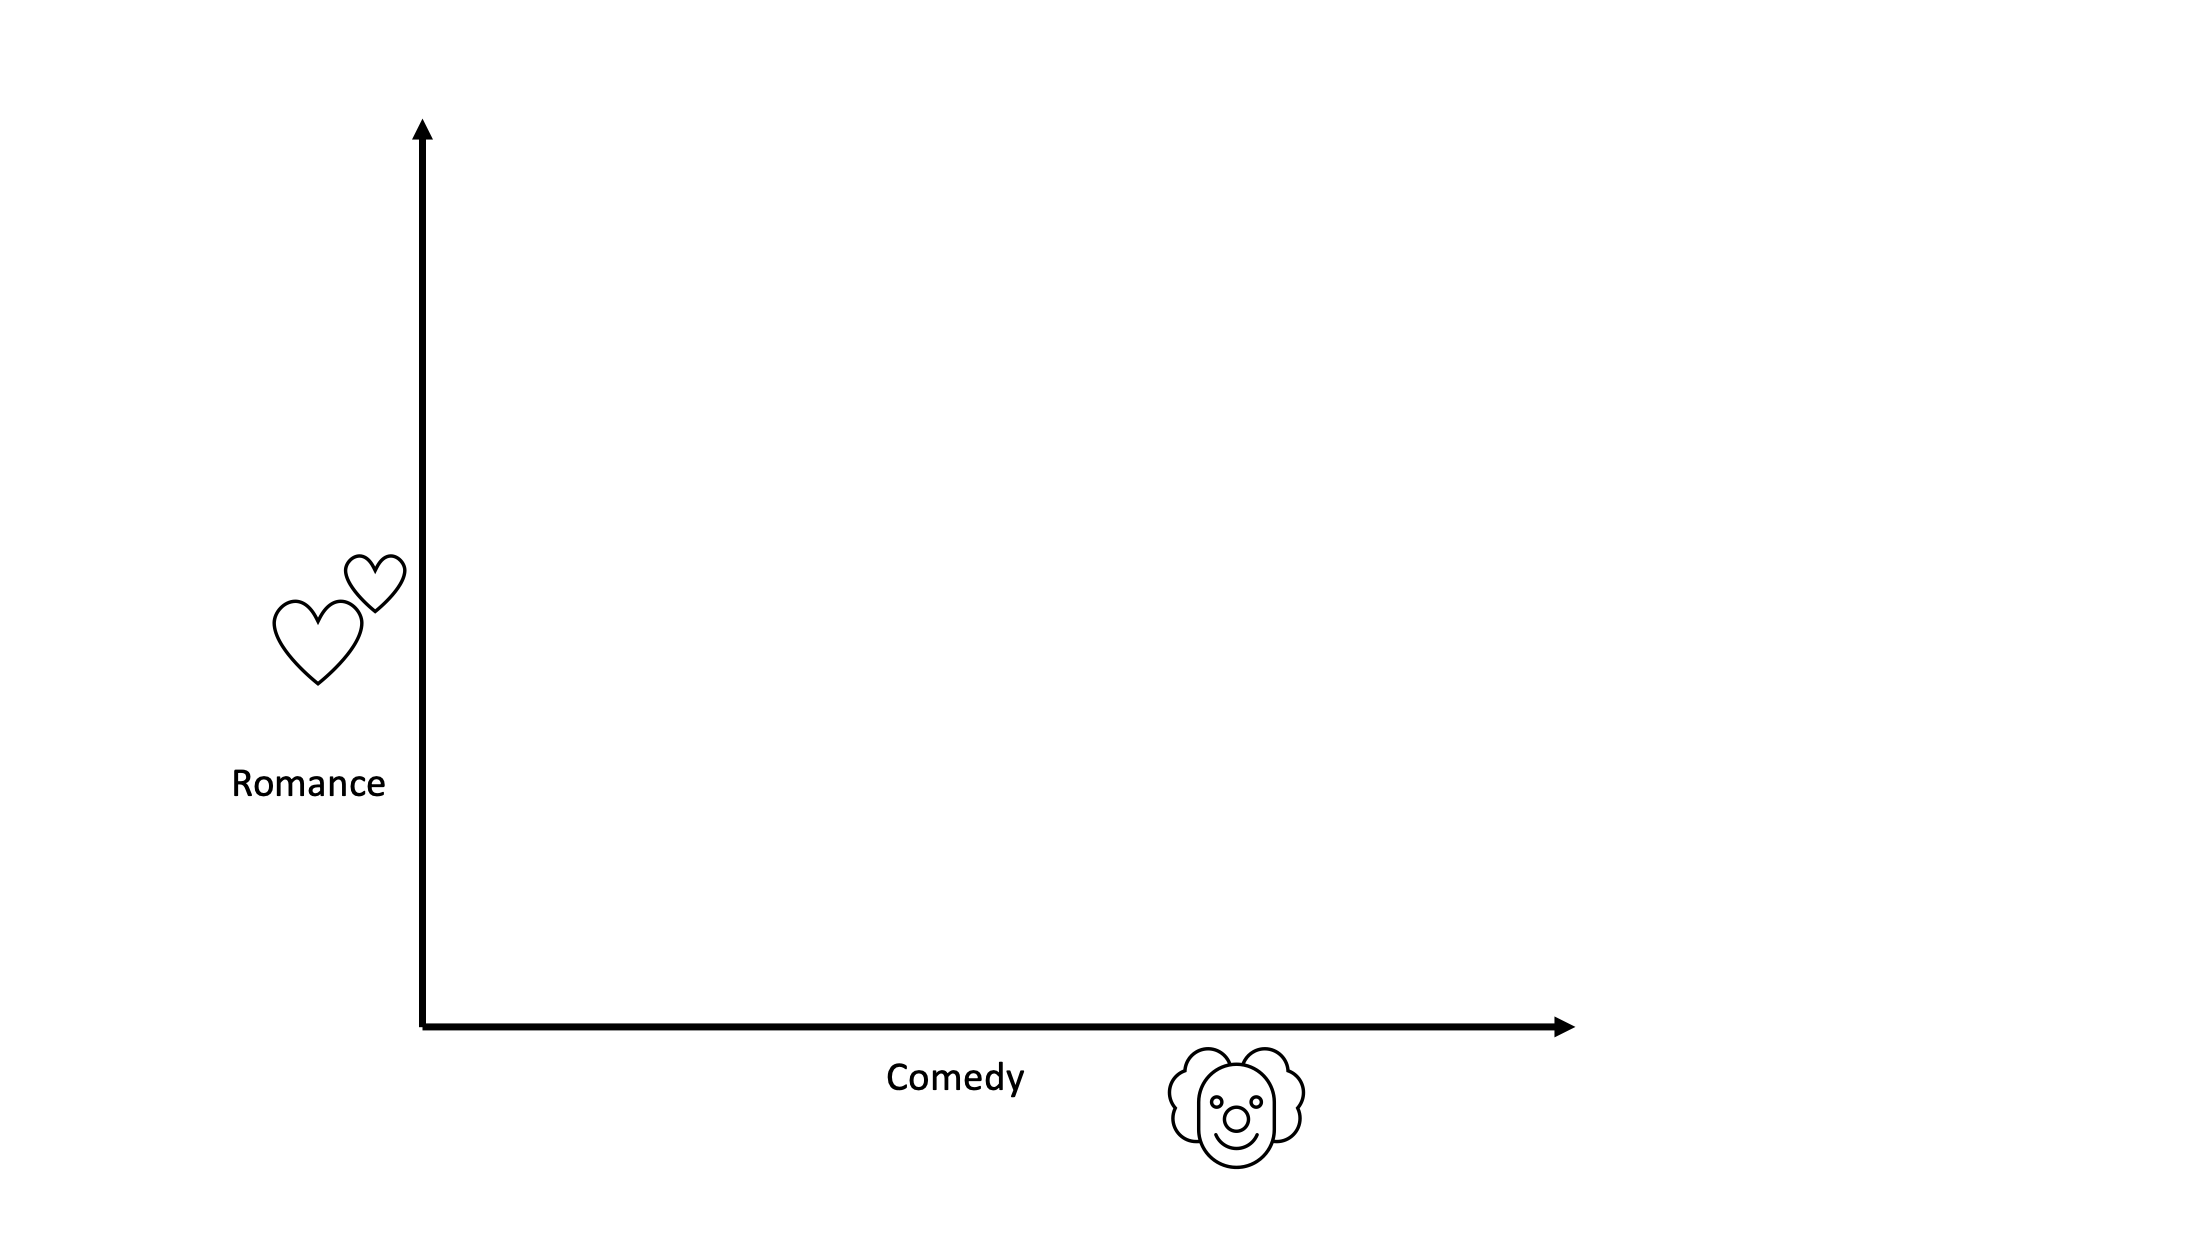
\includegraphics[width=\columnwidth,height=\paperheight,keepaspectratio]{../pictures/Slide1.png}}
\end{frame}

\begin{frame}{Similarity between movies}
	\makebox[\linewidth]{
		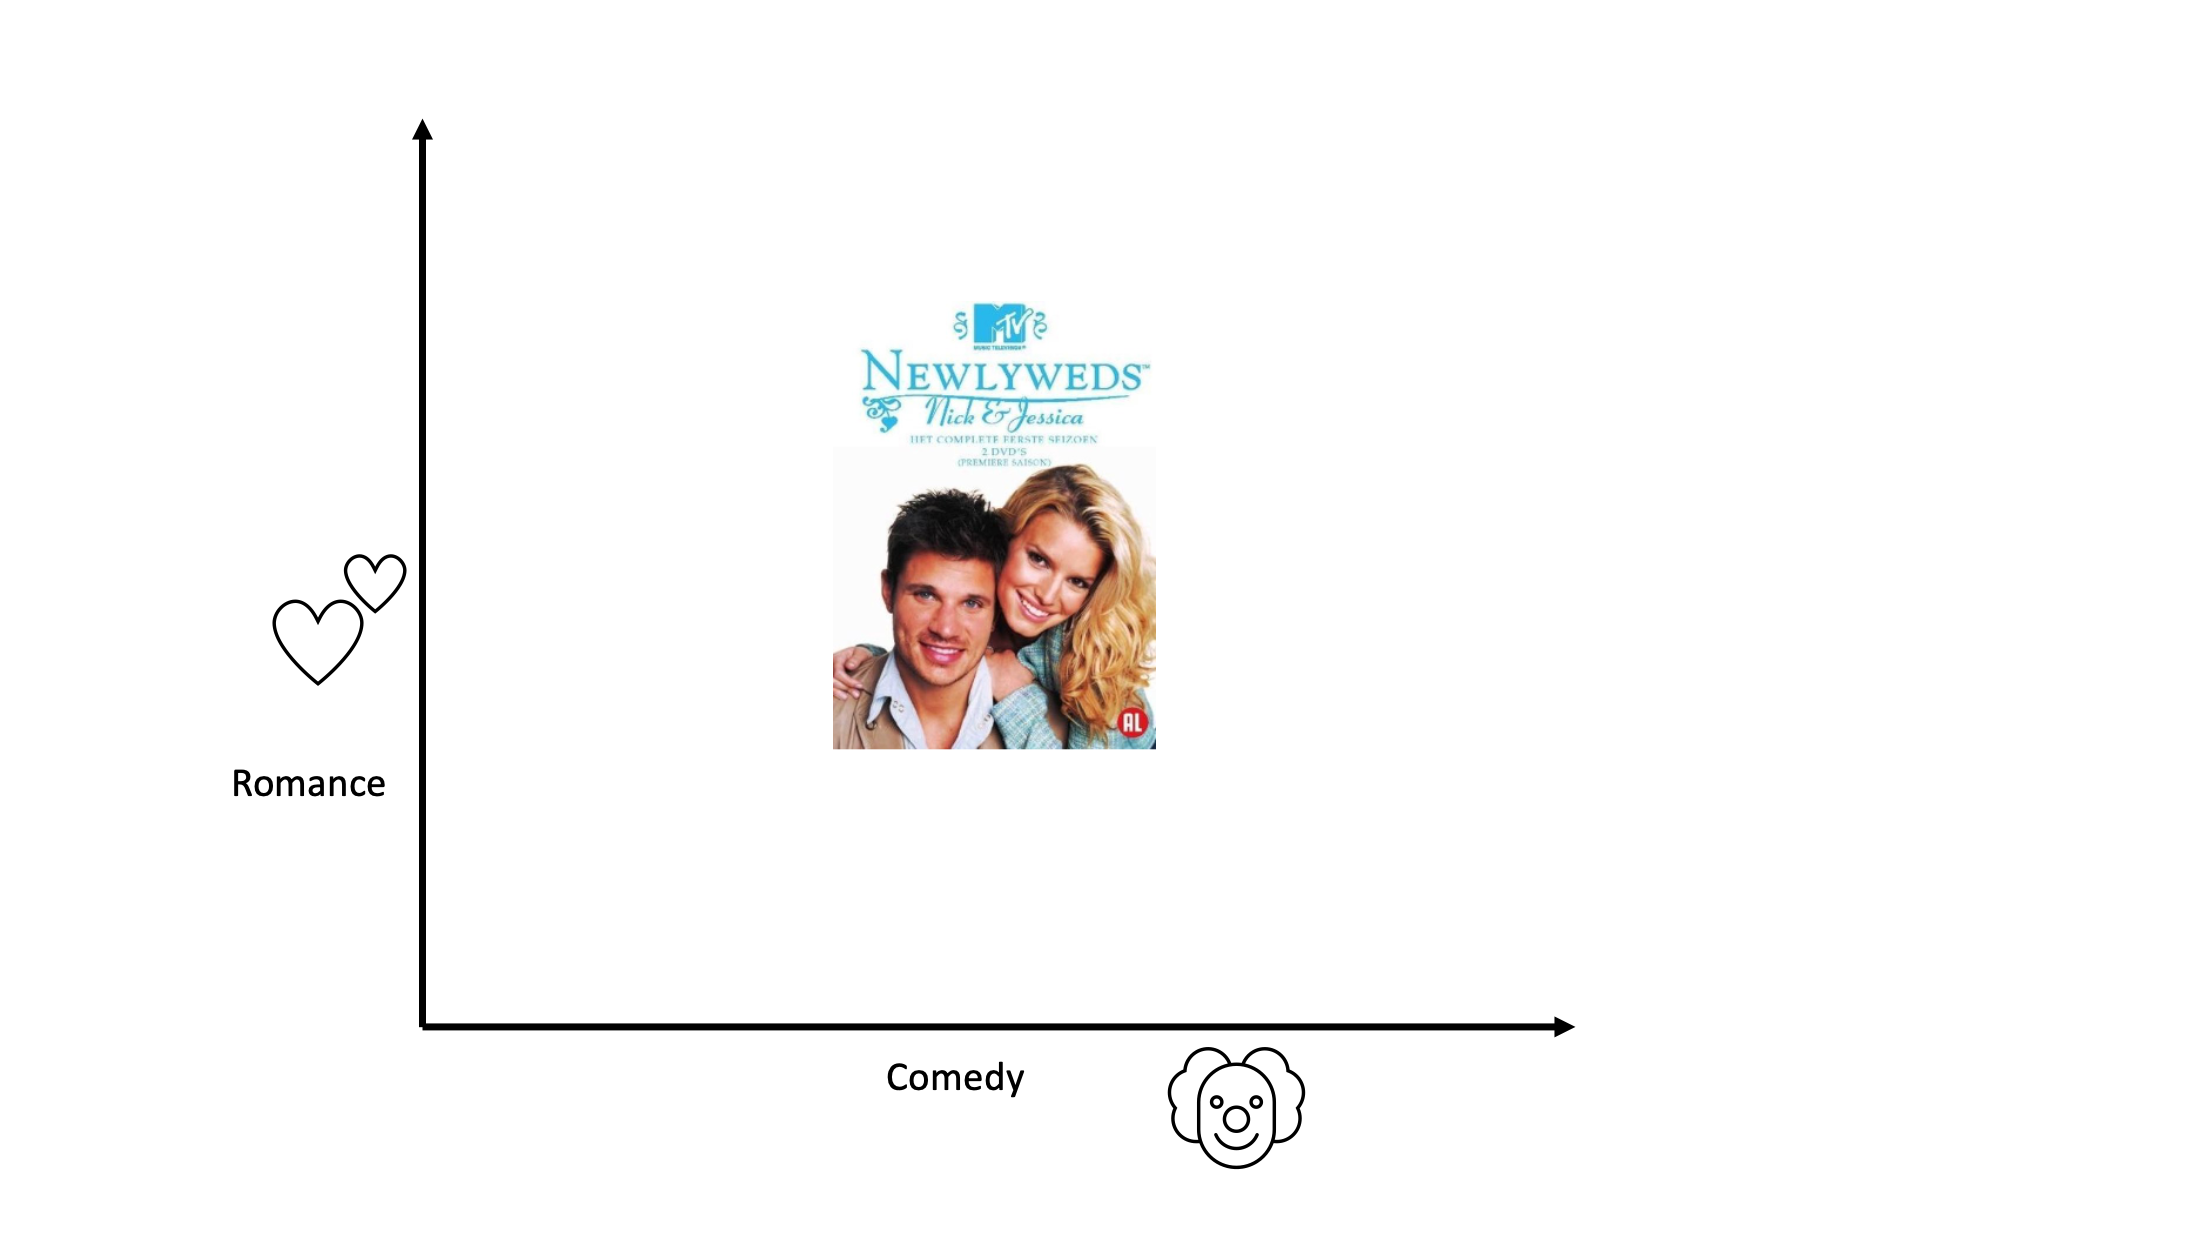
\includegraphics[width=\columnwidth,height=\paperheight,keepaspectratio]{../pictures/Slide2.png}}
\end{frame}

\begin{frame}{Similarity between movies}
	\makebox[\linewidth]{
		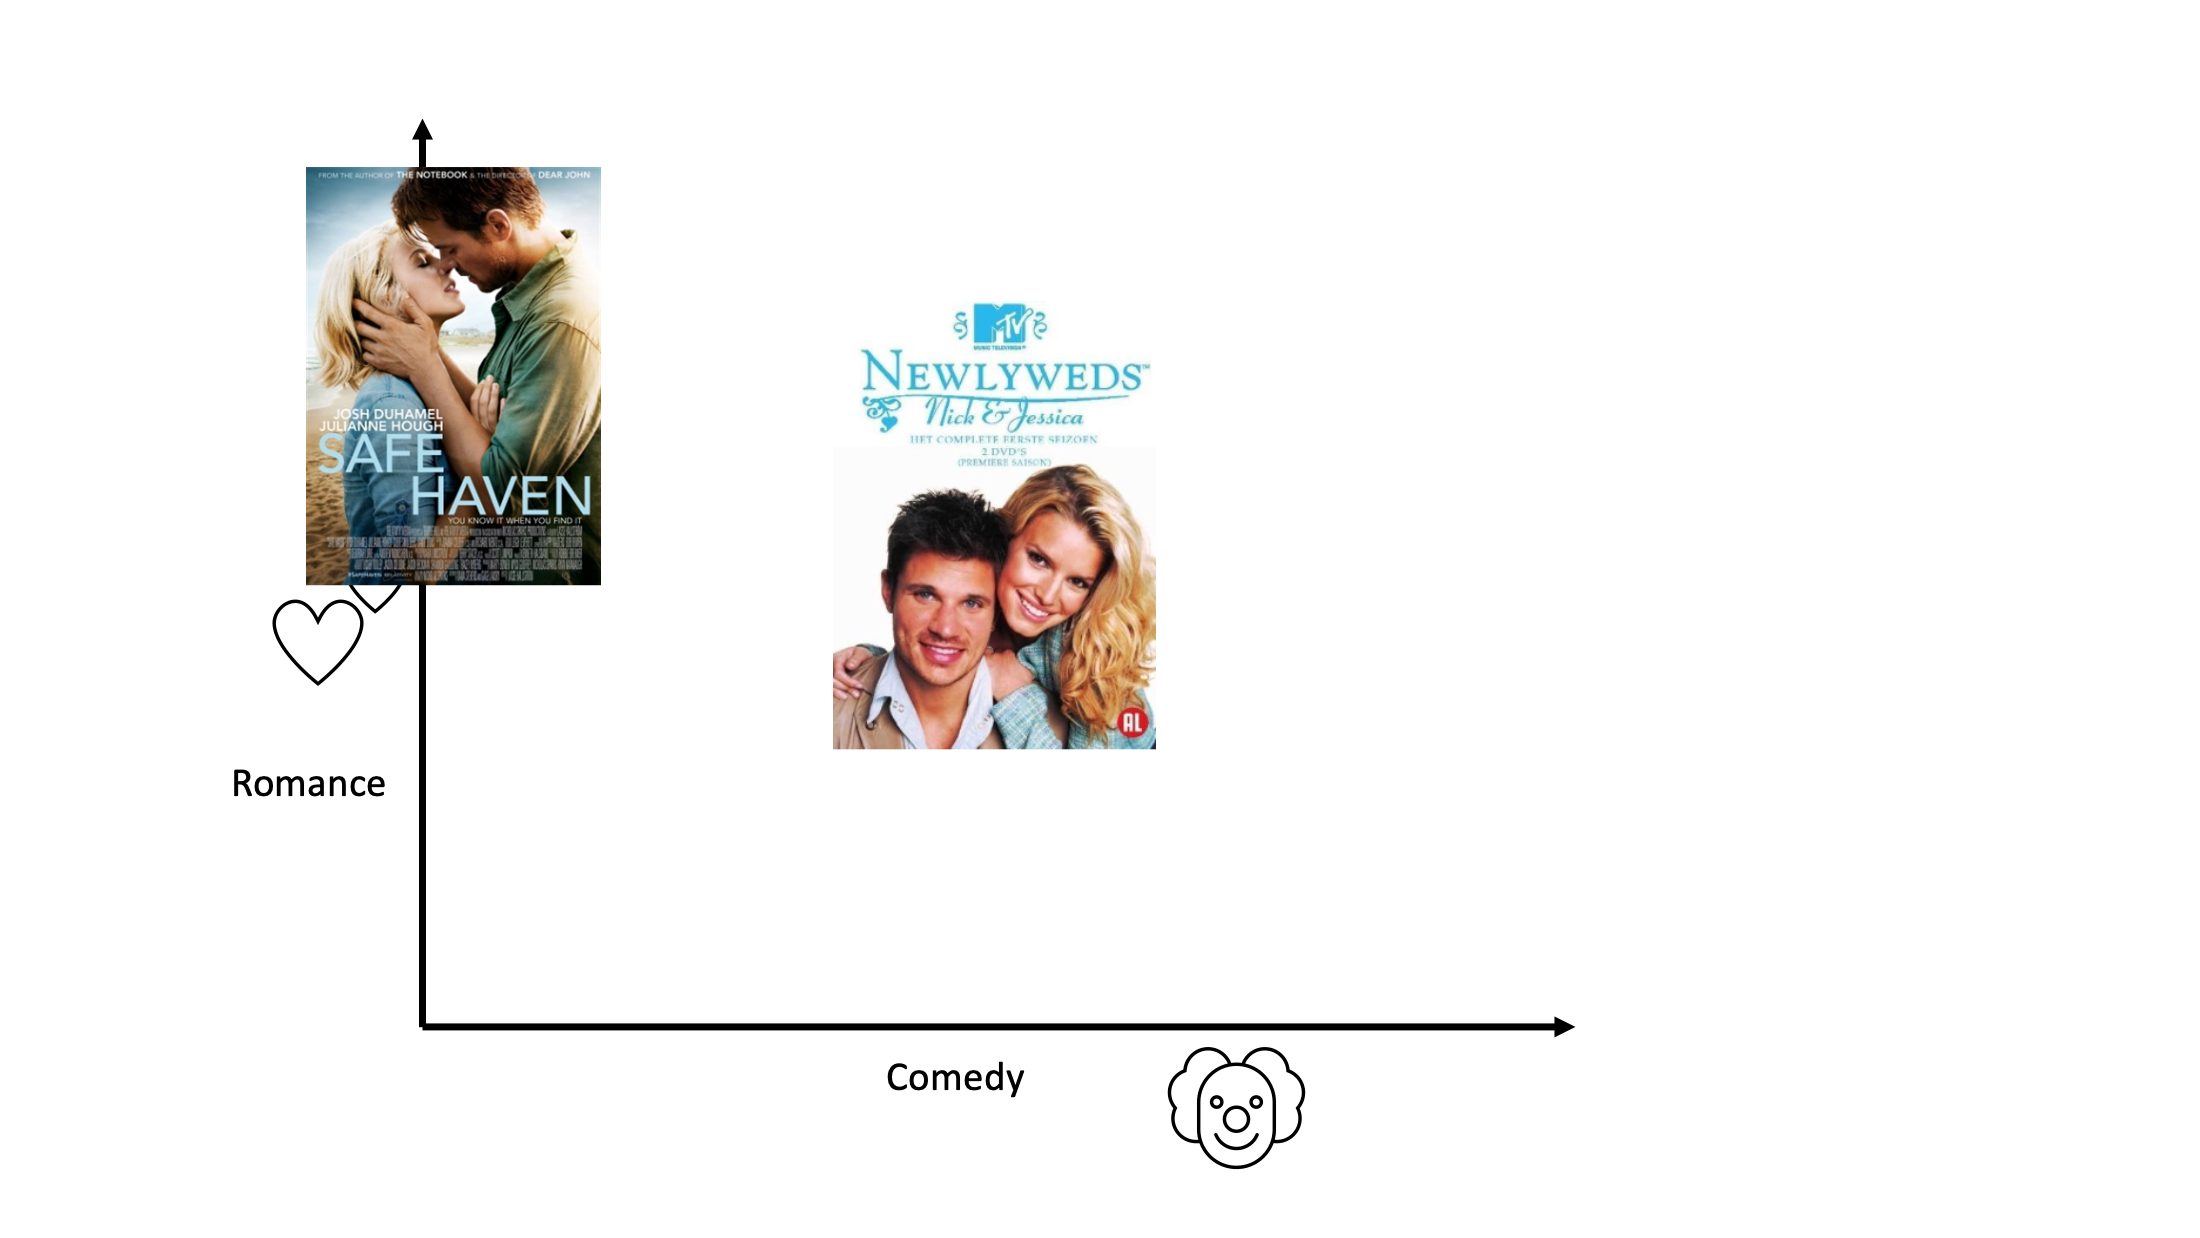
\includegraphics[width=\columnwidth,height=\paperheight,keepaspectratio]{../pictures/Slide3.png}}
\end{frame}

\begin{frame}{Similarity between movies}
	\makebox[\linewidth]{
		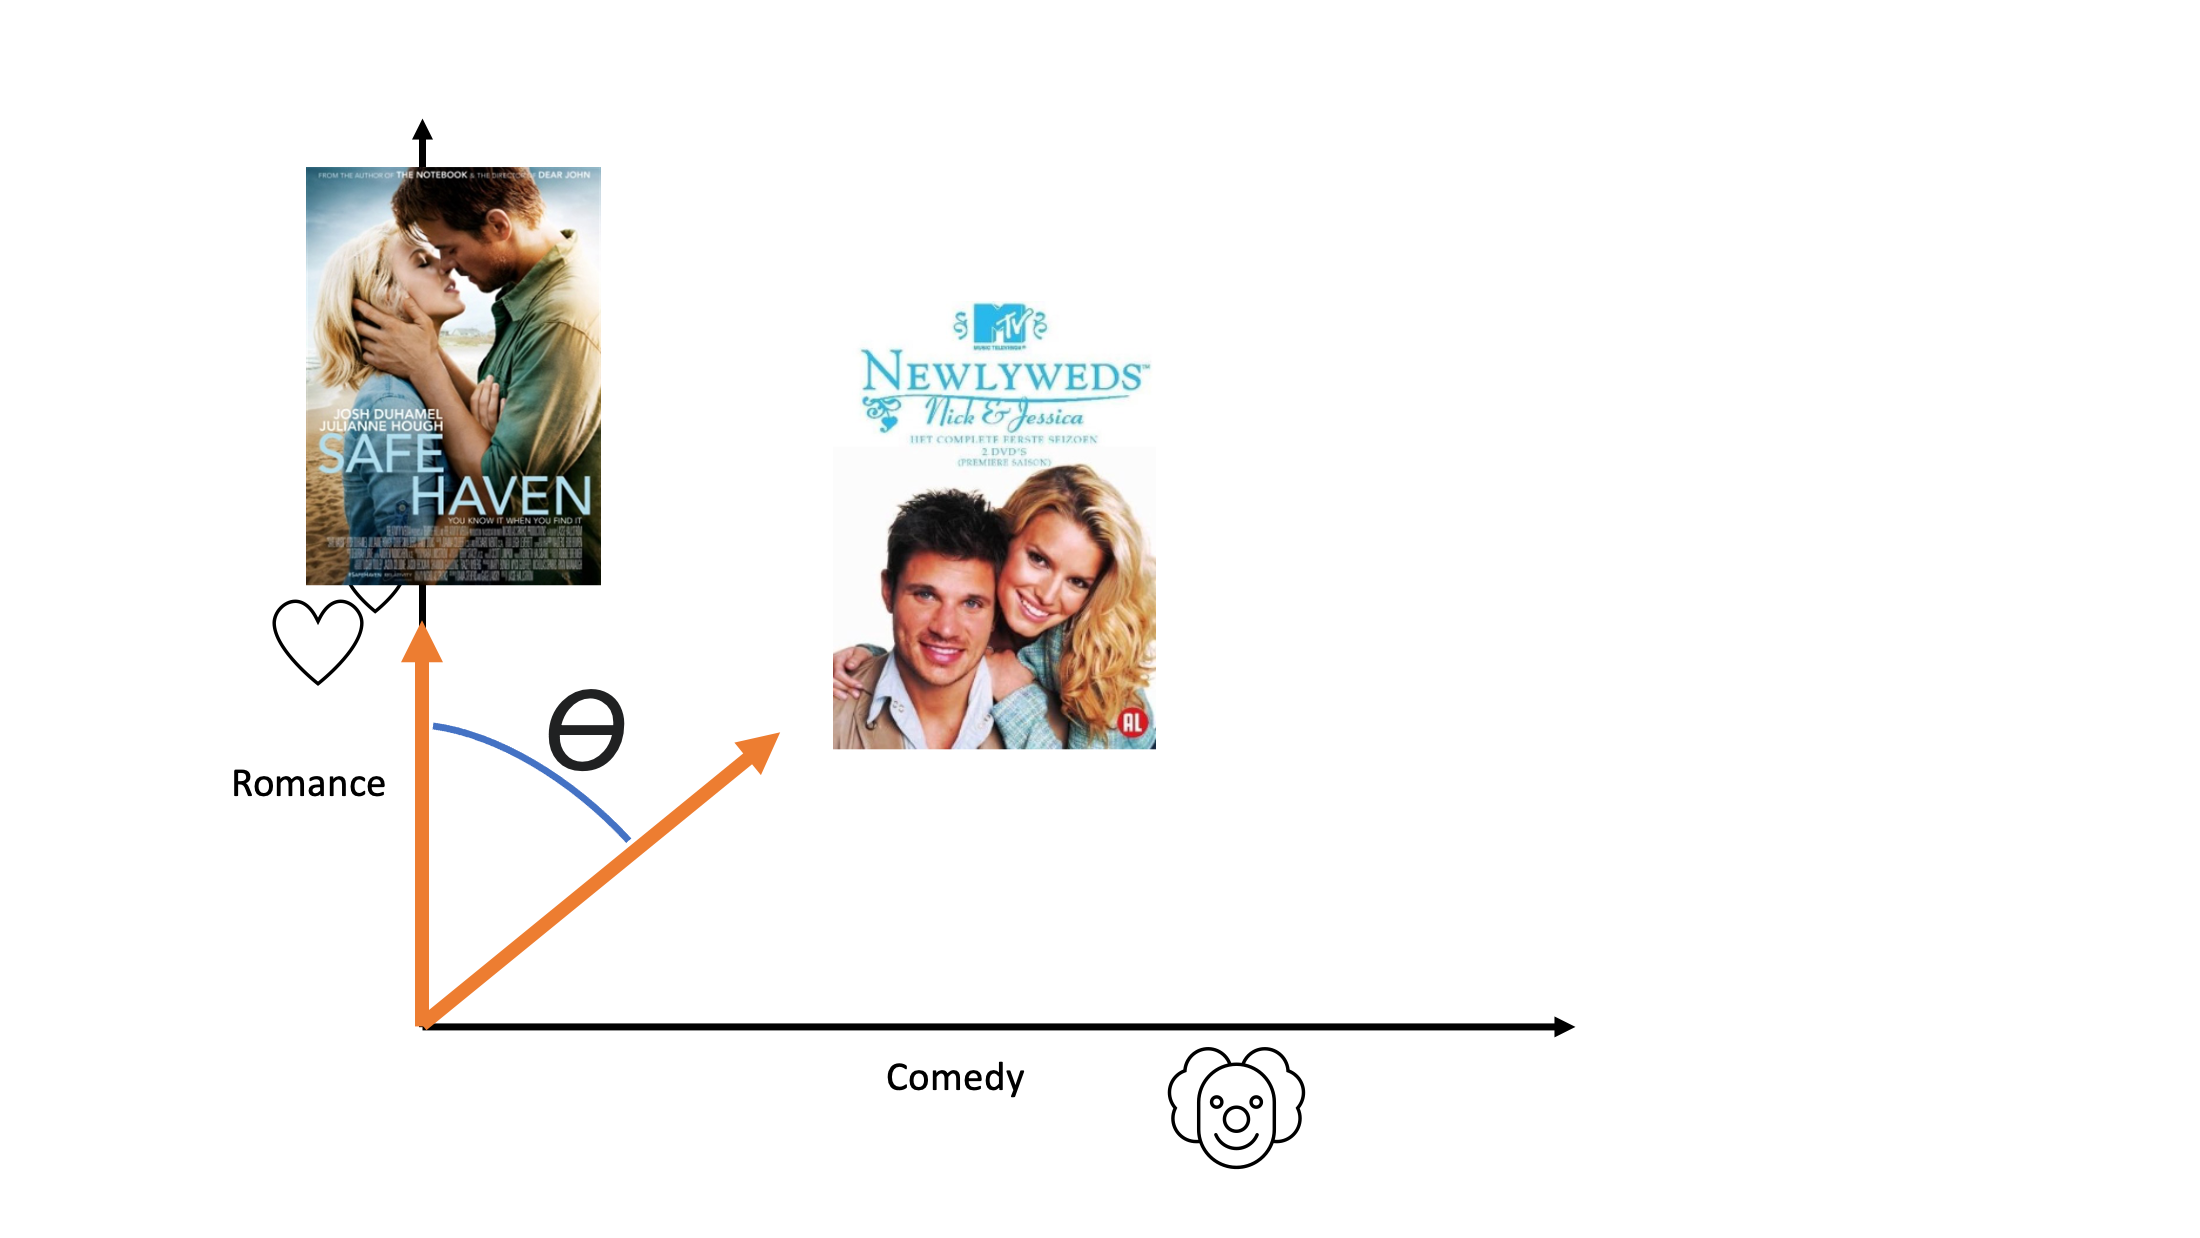
\includegraphics[width=\columnwidth,height=\paperheight,keepaspectratio]{../pictures/Slide4.png}}
\end{frame}

\begin{frame}{Similarity between movies}
	\makebox[\linewidth]{
		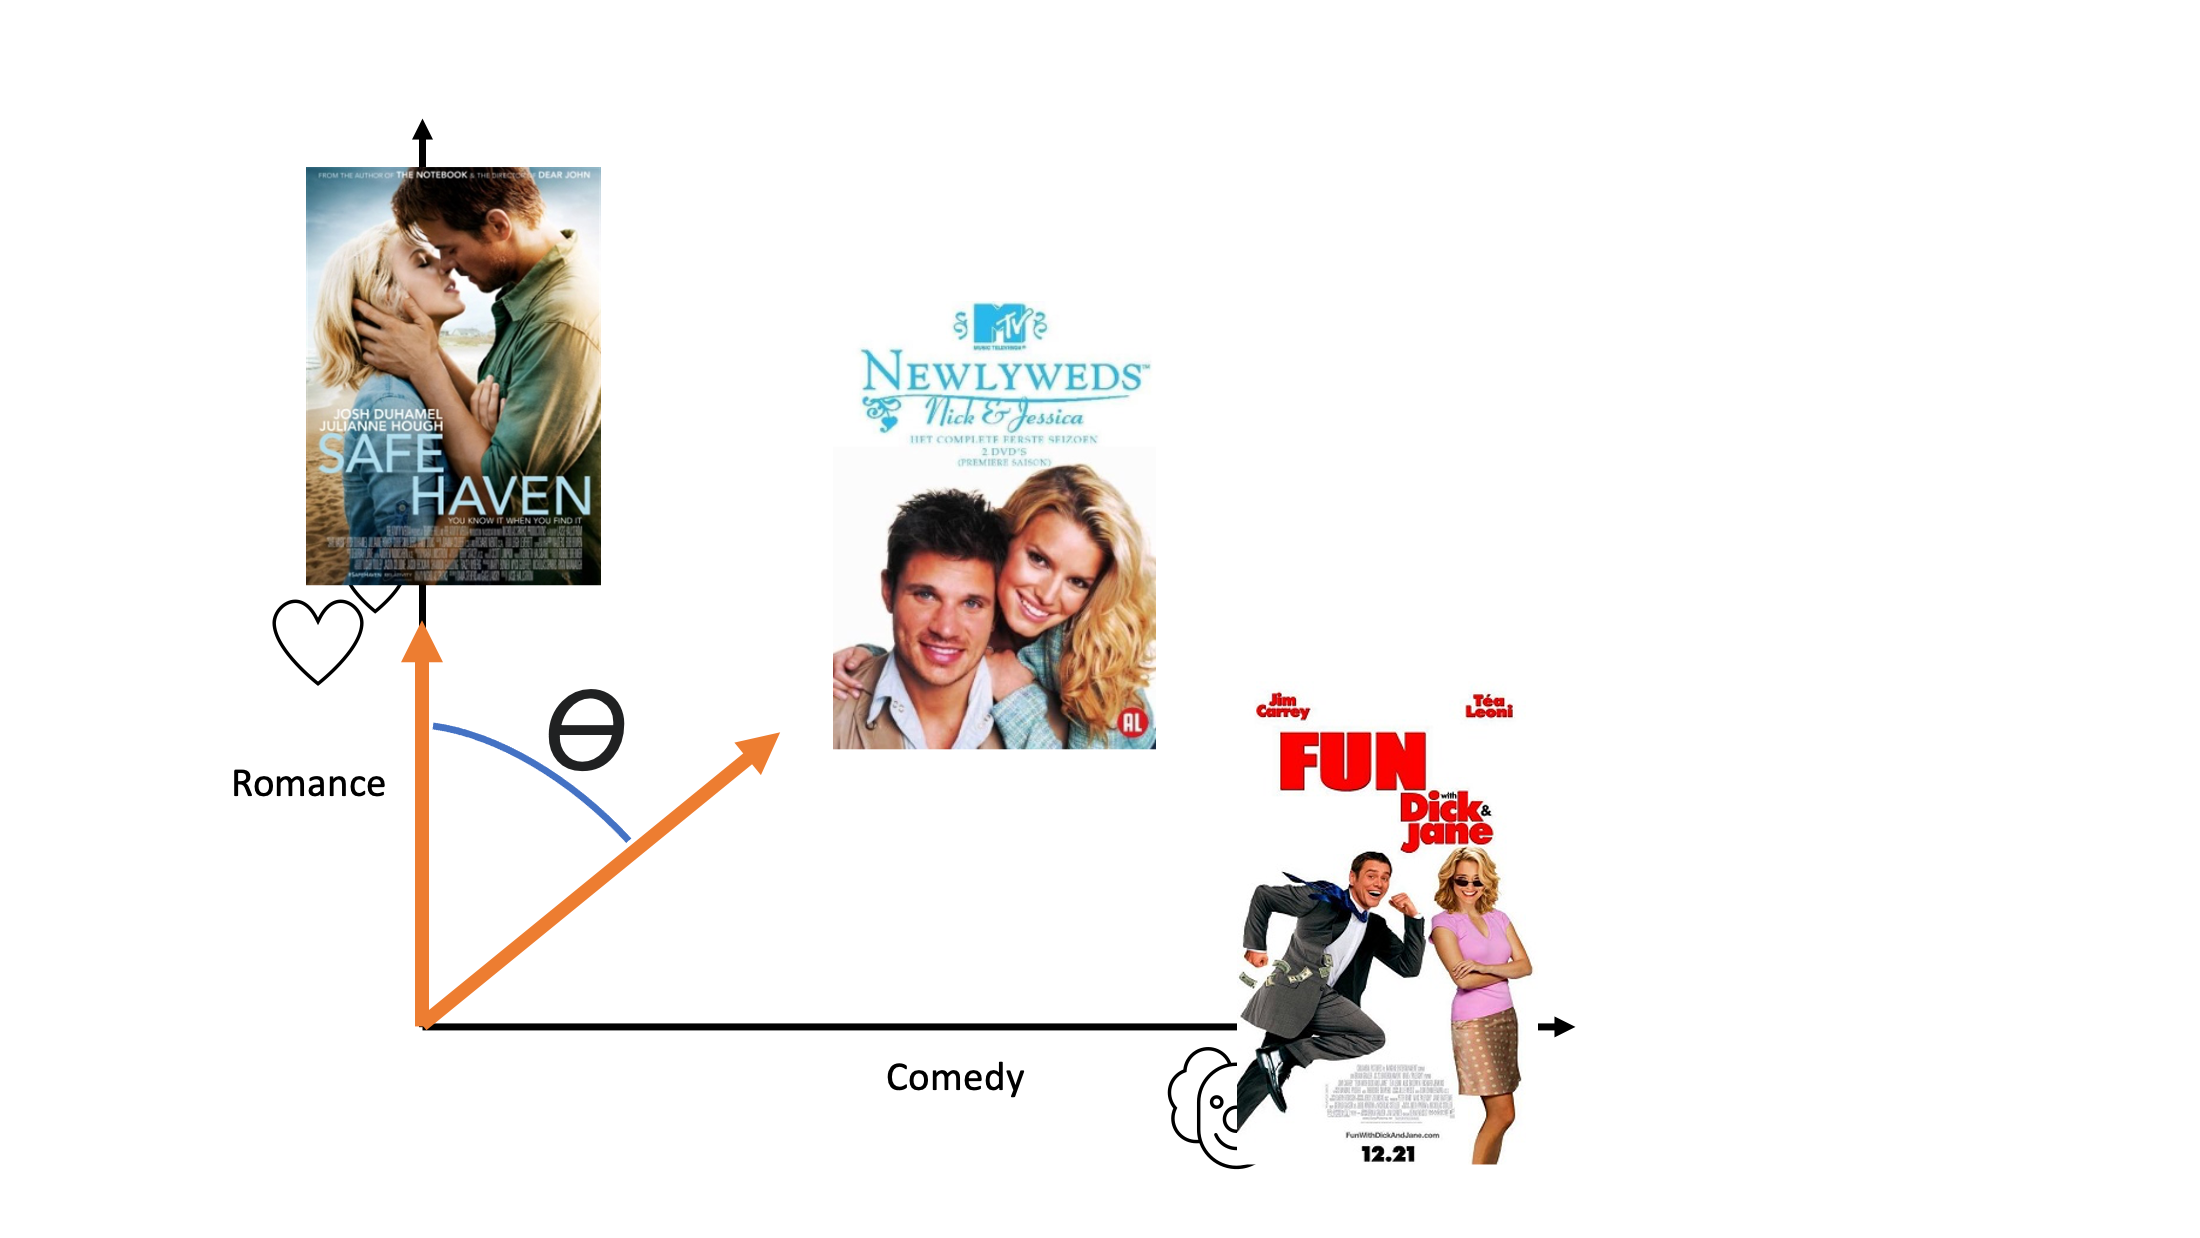
\includegraphics[width=\columnwidth,height=\paperheight,keepaspectratio]{../pictures/Slide5.png}}
\end{frame}

\begin{frame}[fragile]{Let's put this in code!}
	\pause
	First, create a create a toy dataset.
	\pause
	\begin{minted}{python}
data = data.sample(6)
data[['title', 'genres']]
	\end{minted}
	\pause
	\makebox[\linewidth]{
		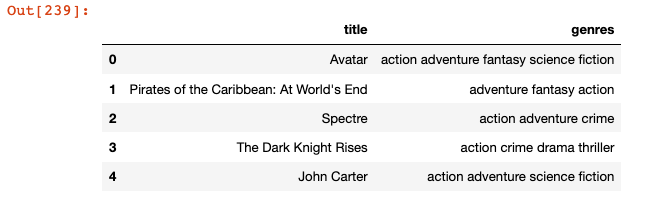
\includegraphics[width=\columnwidth,height=\paperheight,keepaspectratio]{../pictures/toy}}
\end{frame}

\begin{frame}[fragile]{Feature selection and vectorization}
	Let's assume we want to calculate similiarity based on genres. Therefore, we need to vectorize this column. 
	\begin{minted}{python}
tfidf = TfidfVectorizer(stop_words='english')
tfidf_matrix = tfidf.fit_transform(data['genres'])
	\end{minted}
	\pause
Note that we use \alert{tfidf vectorizer} here, but we you might opt for a different one. 
\end{frame}

\begin{frame}[fragile]{Calculate similiarity}
	Now, let's calculate cosine similarity scores between the genre attributes of the movies
	\begin{minted}{python}
from sklearn.metrics.pairwise import cosine_similarity
sim = cosine_similarity(tfidf_matrix)
	\end{minted}
	\pause
This returns an array of the similiarity scores between each movie and all other movies. 
\end{frame}

\begin{frame}[fragile]{Cosine Similairity}
	Let's inspect the output...
\begin{minted}[fontsize=\tiny]{python}
print(sim)
[[1.         0.34503493 0.         0.         0.40824829 0.        ]
[0.34503493 1.         0.16581288 0.         0.28171984 0.29130219]
[0.         0.16581288 1.         0.25964992 0.         0.56921261]
[0.         0.         0.25964992 1.         0.44115109 0.4561563 ]
[0.40824829 0.28171984 0.         0.44115109 1.         0.        ]
[0.         0.29130219 0.56921261 0.4561563  0.         1.        ]]
\end{minted}
\end{frame}


\begin{frame}[plain]
\makebox[\linewidth]{
		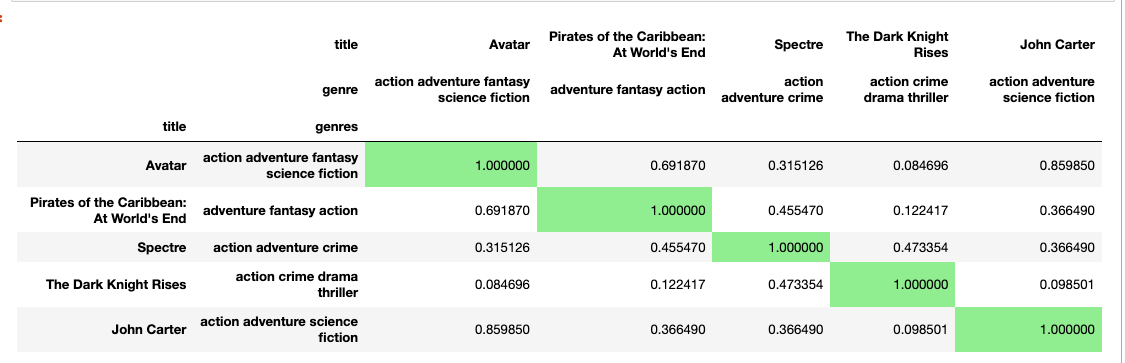
\includegraphics[width=\columnwidth,height=\paperheight,keepaspectratio]{../pictures/cosine_sim}}
	\pause
	Based on this overview, you may assume that users that like \textit{Avatar}, may be interested in \textit{John Carter}. 
		\pause
	\footnotesize{If you want to convert output of \alert{cosine\_similarity} to a \alert{df} type of object, see here \url{https://github.com/uva-cw-ccs2/2223s2/blob/master/week04/exercise/cosine_to_df.md}.}
\end{frame}

\question{Can we automate this proces? Can we automatically find the entry with the most similar movie?}

\subsection*{A more realistic use case}

\begin{frame}{Example of a content-based recsys}
	\makebox[\linewidth]{
		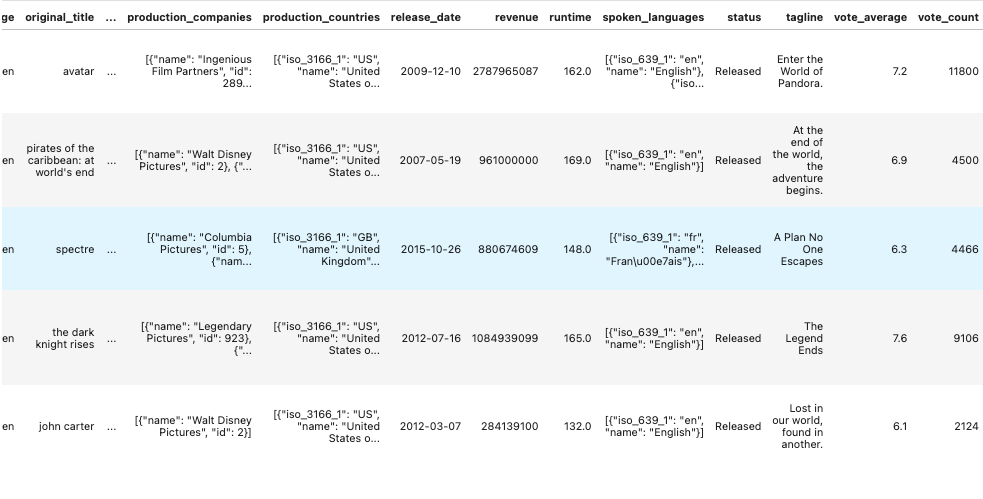
\includegraphics[width=\columnwidth,height=\paperheight,keepaspectratio]{../pictures/dataframe-features}}
\pause
What are interesting features that you can use to base your recommendation on?
\end{frame}


\begin{frame}[fragile]{Get the most similar movies}
First, create an array of cosine scores 
\begin{minted}[%
		breaklines,
		linenos,
		fontsize=\scriptsize,
		frame=single,
		xleftmargin=0pt,]
		{python}
data['combined_features'] = data[['original_title', 'genres', 'overview', 'tagline']].apply(lambda x: ','.join(x.dropna().astype(str)),axis=1)
tfidf = TfidfVectorizer(stop_words='english')
tfidf_matrix = tfidf.fit_transform(data['combined_features'])
cosine_sim = cosine_similarity(tfidf_matrix)
\end{minted}
	\pause
Let's say we want to find the similarity scores associated with the movie \texttt{The Dark Night Rises}. 
\end{frame}

\begin{frame}{Example of a content-based recsys}
	\makebox[\linewidth]{
		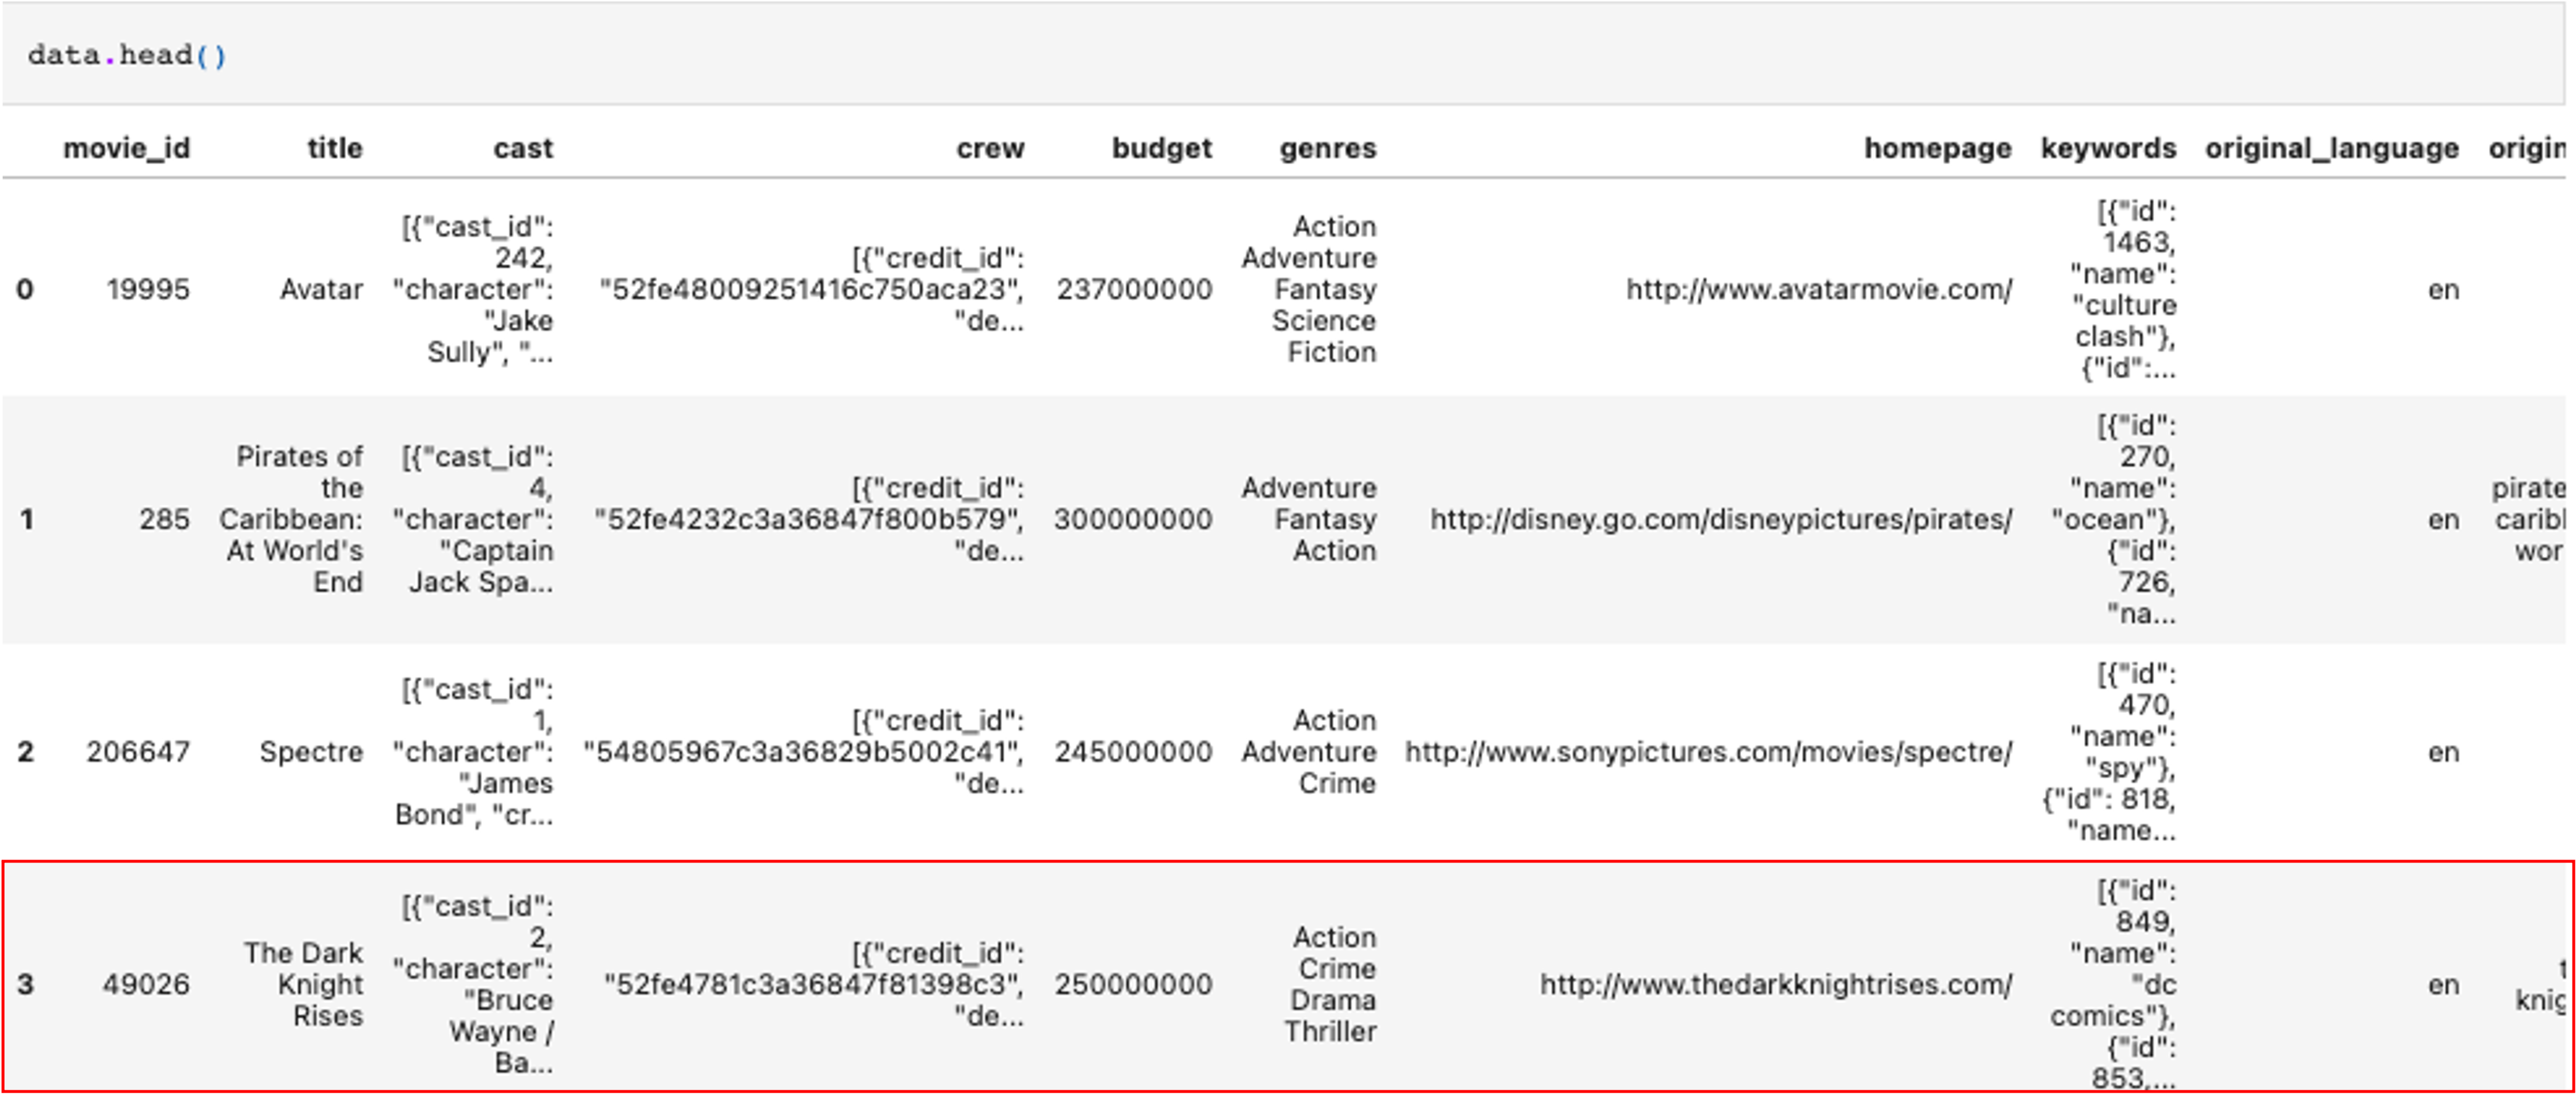
\includegraphics[width=\columnwidth,height=\paperheight,keepaspectratio]{../pictures/df-movies}}
Let's say we want to find the similarity scores associated with the movie \texttt{The Dark Night Rises}. Just by looking at the dataframe, we know it is at index \texttt{3}.
\end{frame}


\begin{frame}[fragile]
\begin{minted}[%
	breaklines,
	linenos,
	fontsize=\scriptsize,
	frame=single,
	xleftmargin=0pt,]
	{python}
cosine_sim[3]
\end{minted}
\pause
\begin{minted}[fontsize=\tiny]{python}
array([0.02331349, 0.00399197, 0.00780174, ..., 0.02860083, 0.03756737, 0.018984  ])
\end{minted}
\pause
A more systematic way to get the index value, is to simple look it up:
\begin{minted}[%
	breaklines,
	linenos,
	fontsize=\scriptsize,
	frame=single,
	xleftmargin=0pt,]
	{python}
indices = pd.Series(data.index, index = data['original_title'])
index = indices['the dark knight rises']
print(index)
\end{minted}
\pause
\begin{minted}[fontsize=\tiny]{python}
3	
\end{minted}
\end{frame}

\begin{frame}[fragile]{Get the most similar movies}
\begin{itemize}
	\item<1->Next, we need to sort the associated vector of cosine similarity scores for this movie to get the most similair movies.
	\item<2->Before sorting the cosine scores, we map the movie-index to the cosine value. We can do so by simple enumerating the cosine scores:
\end{itemize}
\pause
\begin{minted}[%
	breaklines,
	linenos,
	fontsize=\scriptsize,
	frame=single,
	xleftmargin=0pt,]
	{python}
sim_scores = list(enumerate(cosine_sim[index])) 
\end{minted}
\pause
\begin{minted}[fontsize=\tiny]{python}
[(0, 0.023313489832942038),
(1, 0.003991972883233364),
(2, 0.007801739082093903), ...
\end{minted}
\pause
Next, we can simple sort the cosine scores:
\begin{minted}[%
	breaklines,
	linenos,
	fontsize=\scriptsize,
	frame=single,
	xleftmargin=0pt,]
	{python}
sim_scores = sorted(sim_scores, key=lambda x: x[1], reverse=True)
sim_scores = sim_scores[1:11]
\end{minted}
\pause
\begin{minted}[fontsize=\tiny]{python}
[(3, 0.9999999999999998),
(65, 0.3484608502957436),
(299, 0.32460952432731993),
\end{minted}
\end{frame}

\begin{frame}[fragile]{Get the most similar movies}
	And finally look up the associated movies..
	\pause
\begin{minted}[%
	breaklines,
	linenos,
	fontsize=\scriptsize,
	frame=single,
	xleftmargin=0pt,]
	{python}
movie_indices = [i[0] for i in sim_scores]
movie_indices
	\end{minted}
	\pause
	\begin{minted}[fontsize=\tiny]{python}
[299, 1359, 3854, 428, 119, 210, 9, 2507, 979]
	\end{minted}
	\pause
	Map the index values to the dataframe:
\begin{minted}[%
	breaklines,
	linenos,
	fontsize=\scriptsize,
	frame=single,
	xleftmargin=0pt,]
	{python}
data.iloc[movie_indices]['title']
	\end{minted}
	\pause
	\begin{table}[]
		\scalebox{0.7}{
			\begin{tabular}{ll}
299  & Batman Forever                          \\
1359 & Batman                                  \\
3854 & Batman: The Dark Knight Returns, Part 2 \\
428  & Batman Returns                          \\
119  & Batman Begins                           \\
210  & Batman \& Robin                         \\
9    & Batman v Superman: Dawn of Justice      \\
2507 & Slow Burn                               \\
979  & Free State of Jones                    
		\end{tabular}}
	\end{table}
\end{frame}




\subsection*{Building blocks of content-based RecSys}

\begin{frame}
	\begin{block}{Feature selection and engineering}
		\begin{itemize}
			\item Feature engineering is very important here. What qualities or attributes do we want to incorporate?
			\pause
			\item Think about this critically. Instead of using genres or authors, you could think about crafting features yourself, such as topics. 
			\pause
		\end{itemize}
	\end{block}
\end{frame}


\begin{frame}  
	\begin{block}{how can we identify similar items?}
		\begin{enumerate}
			\item<1->Cosine similarity
			\item<2->Soft cosine similarity
			\item<3-> LDA: topic scores
		\end{enumerate}
	\end{block}
\end{frame}

\begin{frame}
	\begin{exampleblock}{Benefits}
		\begin{itemize}
			\item <1-> Content-based recommender systems can be very efficient...
			\item <2->They are often part of more complex recommender systems that leverage (deep) supervised learning
		\end{itemize}
	\end{exampleblock}
	\begin{alertblock}{Drawbacks}
		\begin{itemize}
			\item <3->Features that are not part of the user profile will be neglected; e.g., if the user does not like Super Hero movies, the recommender system wil never recommend this. 
			\item <4->does not use the power community data. Recommendations may be obvious (e.g., \textit{Harry Potter} recommendation when you like \textit{Lord of the Rings})
		\end{itemize}
	\end{alertblock}
\end{frame}

\section[Collaborative RecSys]{Collaborative Recommender Systems}

\begin{frame}{Collaborative filtering}  
\begin{block}{What are collaborative systems?}
	\begin{itemize}
	\item <1-> Tries to overcome some of the limitations of content-based systems
	\item <2->Leverages the power of the community, tries to give relevant, but also suprising recommendations. 
	\item <3-> Very succesful models in industry settings
\end{itemize}
\end{block}
\begin{alertblock}{Types of collaborative systems}
	\begin{enumerate}
		\item User-based collaborative filtering
		\item Item-based collaborative filtering 
	\end{enumerate}
\end{alertblock}
\end{frame}

\begin{frame}{User-based filtering}  
	\begin{block}{Similar users...}
		\begin{itemize}
			\item<1->If we find users that are similar in terms of the things they liked in the past...
			\item<2->...we can use this information to predict what they like in the future
		\end{itemize}
	\end{block}
\end{frame}

\begin{frame}{User-based filtering}
	\makebox[\linewidth]{
		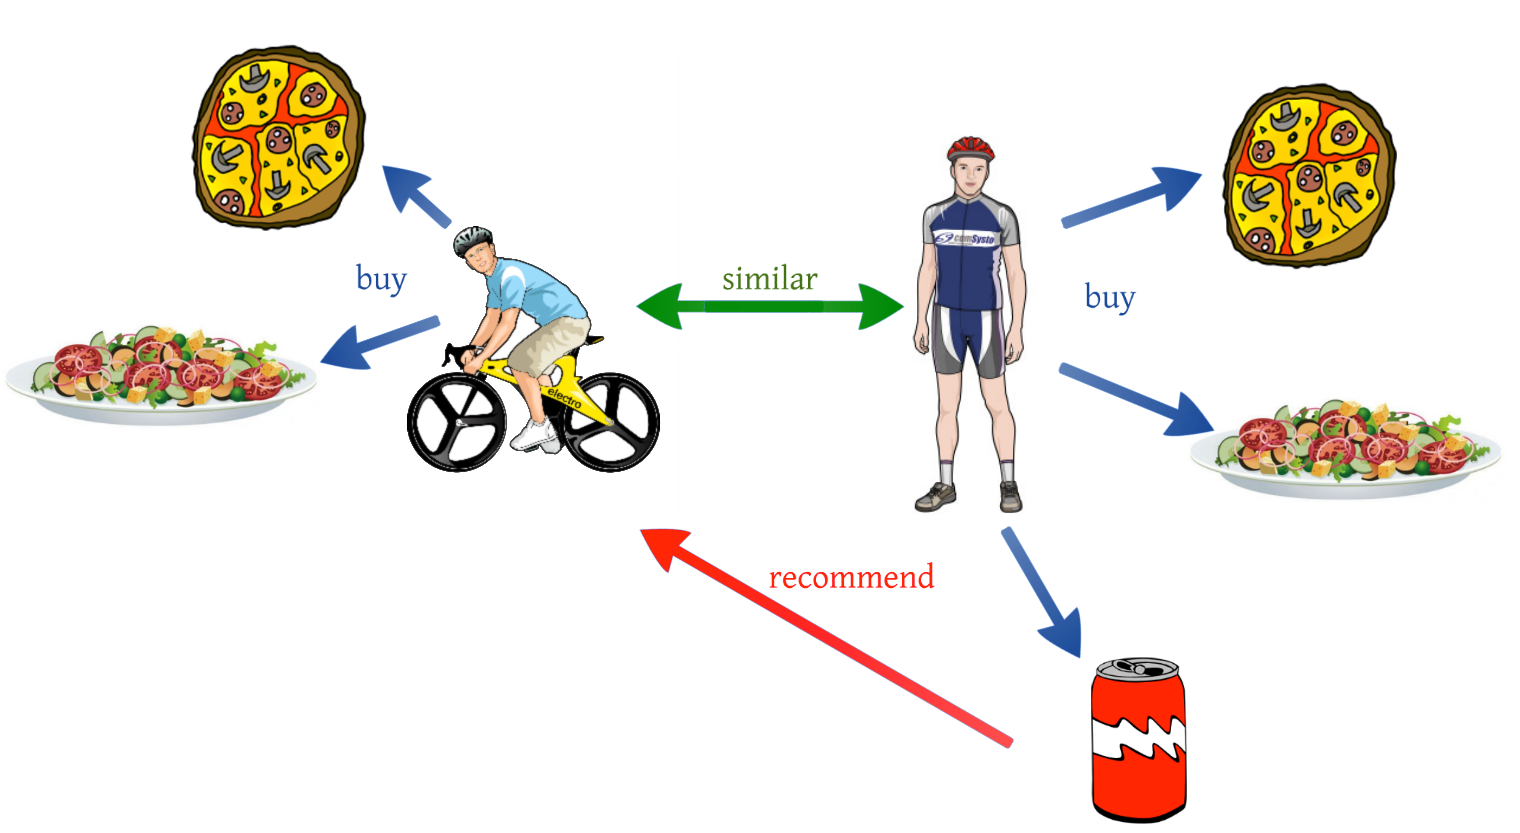
\includegraphics[width=\columnwidth,height=\paperheight,keepaspectratio]{../pictures/collaborative.png}}
	\footnote{Source: \url{https://medium.com/@akhilesh3091999/recommender-system-bb032b16ab67}}
\end{frame}

\begin{frame}{Item-based filtering}  
	\begin{block}{Similar items...}
		\begin{itemize}
			\item<1->If two items is rated similarly by a group of people
			\item<2->...these product might be similar
		\end{itemize}
	\end{block}
		\begin{exampleblock}{Example...}
			\begin{itemize}
			\item If Alex, Sanne and Marthe like skincare product \textit{X} and \textit{Y}, and Denise buys skincare product  \textit{Y},  \textit{X} will be recommended. 
			\end{itemize}
		\end{exampleblock}
\end{frame}

\begin{frame}{User-based filtering}
	\makebox[\linewidth]{
		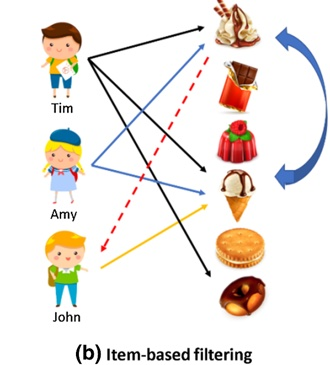
\includegraphics[width=0.5\textwidth]{../pictures/item_based}}
	\footnote{Source: \url{https://predictivehacks.com/item-based-collaborative-filtering-in-python/}}
\end{frame}

\begin{frame}{Example: Amazon}
	\makebox[\linewidth]{
		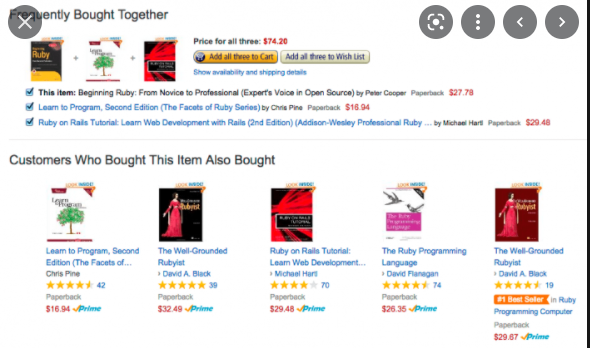
\includegraphics[width=0.5\textwidth]{../pictures/userbased-amazon}}
\end{frame}

%\section[Reflection]{The role of recommender systems in society}

\begin{frame}{Reflection on the role of recommender systems in society}
	\begin{alertblock}{Food for thought}
		\begin{itemize}
			\item <1->Consequences of recommender systems for democratic values in society
		\end{itemize}
	\end{alertblock}
\end{frame}

%\section[Group ass]{Group Assignment}
%\begin{frame}{Build your own recommender system}
%	\begin{alertblock}{Part of the assignment: Build a recommender (20\% of final grade)}
%		\begin{itemize}
%			\item <1->Build a recommender system, based on the insights from this week (week 6). It's up to you to decide whether you build a knowledge-based or content-based recommender system.
%			\item <2->Think about relevant features that you want to use in your algorithm design. Based on which features do you want to recommend content?
%		\end{itemize}
%	\end{alertblock}
%\end{frame}

\begin{frame}{Build your own recommender system}
	\begin{exampleblock}{Practice with the materials!}
		\begin{itemize}
			\item <3-> To be able to do this correctly, it is essential that you understand the code of this week's lab session. 
			\item <4-> Carefully walk through this week's assignment, and to whether questions arise.
			\item <5-> It's up to you to decide whether you want to build a simple knowledge-based or content-based recommender system. Base your selection on the available data columns.
		\end{itemize}
	\end{exampleblock}
\end{frame}